\documentclass[pageno]{jpaper}
% \DeclareSymbolFont{letters}{OML}{ztmcm}{m}{it}
% \DeclareSymbolFontAlphabet{\mathnormal}{letters}

% Change to current semester and year, e.g.:
% \newcommand{\IWreport}{Spring 2020}
\newcommand{\IWreport}{Spring 2023}
\newcommand{\quotes}[1]{``#1''}
\newcommand{\lb}{\; | \;}
\newcommand{\tsteps}{\Mapsto_{\textrm{t}}}
\newcommand{\esteps}{\Mapsto_{\textrm{e}}}
\newcommand{\spacedot}{\; . \;}
\newcommand{\spaced}[1]{\; #1 \;}
\newcommand{\s}{\mathbb{S}}
\newcommand{\typrule}[3]{\frac{#1}{#2} \ \textbf{#3}}
\newcommand{\gamimp}{\Gamma \vdash}
\newcommand{\evalrule}[4]{\frac{#1}{#2} \ \boldsymbol{#3}_{\textbf{#4}}}
\newcommand{\env}{\mathtt{env}}
\newcommand{\prob}{\mathtt{prob} \ }
\newcommand{\angles}[1]{\langle #1 \rangle}
\newcommand{\parens}[1]{\llparenthesis #1 \rrparenthesis}
\newcommand{\evalenv}[1]{\langle \env, #1 \rangle}
\newcommand{\mt}[1]{\mathtt{#1}}
\newcommand{\rulename}[2]{$\boldsymbol{#1}_{\textbf{#2}}$}

\makeatletter
\def\verbatim@font{\linespread{1}\normalfont\ttfamily}
\makeatother

\widowpenalty=9999

\usepackage[normalem]{ulem}

\pagestyle{fancy}
\fancyhead[L]{D. Friedman}
\fancyhead[C]{\textbf{IW Report: Implementing ProbaML}}
\fancyhead[R]{Spring 2023}

\begin{document}
\thispagestyle{empty}

\title{
  ProbaML: Implementation of a Functional Language Supporting Probabilistic Computation}

\author{Daniel Friedman\\\textbf{Adviser:} David Walker}

\date{}
\maketitle

\thispagestyle{empty}
\doublespacing

% This paper presents the design, operational semantics, and implementation of a new functional programming language that supports probabilistic features such as sampling from distributions and computing expectations. The language is built with a lexer, parser, and type-checker, and supports the expression of probability distributions and operations on them while minimizing side effects. This project is innovative in its development of a new language that combines the benefits of functional programming and probabilistic computation. The implementation also provides a clear and concise example of how to build an interpreter from the ground up, making it a useful tool for teaching functional programming concepts. Additionally, the paper discusses the background work on functional probabilistic programming and highlights the importance of this project in advancing the field. The language's ease of reasoning about programs and functions without side effects can help simplify the complexity of code and improve the efficiency of probabilistic computations.

\begin{abstract}
  This paper presents the design and implementation of a new functional probabilistic programming language, ProbaML. It supports standard functional features in addition to probabilistic ones such as sampling from probability distributions. This project aims to develop a simple language that combines the benefits of functional programming and probabilistic computation, and presents an introduction to interpreters, functional languages, and probabilistic features to those new to the field. The implementation provides a clear and concise example of how to build a functional language from the ground up. The language is built to make reasoning about programs, functions, and probabilistic features easier due to the minimal side effects and simplicity of the language.
\end{abstract}

\tableofcontents

\section{Introduction}
Functional programming languages have become increasingly popular in recent years due to their ability to reason about complex computations by using functions without side effects. This is especially important in probabilistic computations, which are inherently difficult to reason about due to the presence of randomness. In this paper, we present the design, operational semantics, and implementation of a custom functional language that supports probabilistic features such as sampling from distributions and computing expectations.

Probabilistic programming has gained significant attention in recent years due to its many applications in machine learning and artificial intelligence, robotics, and a variety of other fields. In addition, it is well suited for programs involving probabilistic computations and uncertainty. However, writing probabilistic programs can be challenging because they involve reasoning about random variables and their relationships. Functional programming paradigms have been shown to be well-suited for probabilistic programming because they provide a natural way to express computations involving randomness without side effects, enabling the programmer to write less error-prone code.

In this project, we explain the design and implementation of a custom functional language, \textbf{ProbaML}, that supports probabilistic features while utilizing the functional paradigm. The language includes support for expressing probability distributions and operations on them, as well as the ability to compute expectations. We believe that this language can be a useful tool for researchers and practitioners in the field of functional probabilistic programming.

Furthermore, the implementation of the language will provide a clear and concise example of how to build an interpreter from the ground up. This can be a valuable resource for students learning about functional programming concepts and language implementation. Overall, we believe that this project can contribute to the development of new and more efficient probabilistic programming languages and tools.

\section{Background and Related Work}
There has been a lot of work in the field of probabilistic programming, including that of functional probabilistic programming. The functional paradigm for probabilistic languages is especially useful when reasoning about complex computations or data structures \cite{functional_pearls}. In imperative languages, debugging such implementations would be especially difficult due to the use of functions modifying global state or potentially unexpected interactions between different parts of the program due to side effects. As the uses of probabilistic data structures and other types of probabilistic analysis continue to grow, it becomes increasingly important to design languages and programming paradigms that make it easier to write bug-free code and reason about its correctness.

Previous iterations of functional probabilistic programming often consist of libraries build upon an established functional language such as Haskell or OCaml and libraries like Hakaru and Hansei. As such, they incorporate many complex and advanced features, and are not well suited for beginners or those looking for an introduction to functional programming or probabilistic features.

ProbaML is designed to be an introductory functional language with a core set of features to allow for high expressiveness and functionality, while teaching the basics of probabilistic programming. In addition, the lexer and parsers in the language, as well as the type checker and evaluation relation are meant to provide a clear and concise example of how to build an interpreter for a functional programming language from the ground up. This can be a valuable resource for students and researchers who are interested in learning about functional programming concepts and language implementation.

\section{Approach}
The implementation of ProbaML relies heavily on the work of Park, Pfenning, and Thrun \cite{pfenning_short,pfenning_long}. In these two papers, they describe the design and mathematical basis of a probabilistic functional language, $\lambda_{\circ}$, whose mathematical basis is sampling functions. They use work from previous authors such as Pfenning, Davies, and Moggi \cite{pfenning_davies_2001,moggi,park_calc_prob} to incorporate the lambda calculus into a monadic metalanguage, which serves as the mathematical foundation for $\lambda_{\circ}$. They present the typing judgments and evaluation rules for the language, as well as type safety in the form of proving that progress and type preservation hold in $\lambda_{\circ}$. They also present an implementation of the language in OCaml, using a preprocessor to extend the standard OCaml syntax.

The lambda calculus is especially well suited for an implementation of ProbaML due to its high expressiveness with only a few basic constructs such as functions and variables. As a result, it is a good educational tool to introduce functional programming with a reasonable learning curve.

The approach of Park et al. uses a somewhat outdated preprocessor (CAMLP4), and they choose to build their language on top of the preexisting OCaml framework. This allows them to focus on the probabilistic features as the central features of their work. In this implementation, we choose to start from the parsing stages and incrementally build up to a point at which we can add both standard functional features in addition to the probabilistic ones. In this way, we can include probabilistic features as a fundamental construct in the language just like functions, variables, and other terms.

Furthermore, this approach makes several design decisions that differ from those of Park et al. For example, we choose to use the environment model for evaluation (instead of the substitution model) and big-step operational semantics instead of the ones described in their paper. Many other design decisions make ProbaML distinct from $\lambda_{\circ}$.

The approach below also makes use of several resources from the Clarkson textbook \cite{cs3110_book}. In addition, we also use similar features to those presented in the Interpreters Assignment on the COS326 Course Site \cite{cos326_site}.

\section{Implementation}
The implementation of ProbaML is divided into several parts. First, we describe the abstract syntax for the language, its terms, expressions, and other components. Next, we describe the typing rules for ProbaML, and present an implementation of the type-checker in OCaml. We then proceed to describe the operational big-step semantics for the language, as well as the implementation of the evaluation in OCaml. We present two clients, a read-eval-print-loop and an evaluator to repeatedly compute a probabilistic sampling.

\subsection{The Abstract Syntax of ProbaML} \label{abstract_syntax_probaml}
We begin by describing the abstract syntax for ProbaML. These are the fundamental building blocks that we will use for describing the evaluation rules and typing derivations. Figure~\ref{fig:abstract_syntax} summarizes the abstract syntax, including the terms, expressions, values, and sequences in the language.

In addition to supporting standard types such as integers and Booleans, the languages supports the $\square \ A$ type which represents a probability distribution of type $A$. Furthermore, the abstract syntax makes a distinction between \emph{terms} and \emph{expressions}. Terms describe purely deterministic computations that always evaluate to the same value. Expressions describe probabilistic computations. As we describe in Section~\ref{probabilistic_eval_rules}, the values of these probabilistic expressions depend on their \emph{sampling sequences}, and varying these sequences can cause the result to vary as well. We will describe this in more detail later on.

The abstract syntax also includes the sampling expression $\s$, which can be thought of a function that, when given an \emph{infinite sampling sequence} $\omega$, returns the first entry of that sequence which is a uniformly random number in $[0, 1)$. In this way, the $\s$ expression always produces the same value given the same sampling sequence $\omega$, which is an important feature of the language which we describe further in Section~\ref{sampling_function_rand}.

\begin{figure}[hbt]
  \fbox{
    \parbox[c]{\textwidth}{
      \centering
      \begin{align*}
         & \textrm{type}                & A      & ::= A \rightarrow A \lb \square \ A \lb \text{real} \lb \text{int} \lb \text{bool} \\
         & \textrm{term}                & M,N    & ::= x \lb \lambda x:A.M \lb M M \lb \textrm{let } x = M \textrm{ in } N            \\
         &                              &        & \qquad \lb \textrm{prob } E \lb r                                                  \\
         & \textrm{expression}          & E      & ::= M \lb \textrm{sample } x \textrm{ from } M \textrm{ in } E \lb \s              \\
         & \textrm{value}               & V      & ::=  \lambda x:A.M \lb \textrm{prob } E \lb r                                      \\
         & \textrm{real number}         & r      &                                                                                    \\
         & \textrm{variable}            & x      &                                                                                    \\
         & \textrm{sampling sequence}   & \omega & ::= r_1 r_2 \cdots r_i \cdots \quad \textrm{where $r_i \in (0.0, 1.0]$}            \\
         & \textrm{typing context}      & \Gamma & := \cdot \lb \Gamma \lb \Gamma, x:A                                                \\
         & \textrm{dynamic environment} & \env
      \end{align*}
      \caption{Abstract syntax for ProbaML.}
      \label{fig:abstract_syntax}
    }}
\end{figure}

\subsection{Typing Rules} \label{typing_rules}
As mentioned above, one of the key motivations for the creation of the language is that we can formalize its typing rules to ensure type safety. While we do not present the proofs for the type safety of ProbaML here, the typing rules can at least rule out many bugs at compile time, and give the user more detailed error messages before they run the program. Since some expressions in ProbaML are probabilistic, it is especially significant to describe such judgments for probabilistic computations. By describing the typing judgments for probabilistic computations as well, we can make these expressions type-safe as well, making it easier to reason about the execution of these expressions.

The expression type, is evaluated in a \emph{static typing context}, $\Gamma$. This context binds variable names to their associated types. We use the notation $\Gamma \vdash x:A$ to mean that a typing context $\Gamma$ proves that the variable $x$ has type $A$ in $\Gamma$. We use the shorthand notation $\vdash x:A$ to mean $\forall \ \Gamma, \Gamma \vdash x:A$. In addition, we use $\Gamma,x:A$ to mean $\Gamma$ \emph{extended} with the variable $x$ bound to type $A$.

We begin by presenting the typing rules for deterministic terms, and then proceed to present those for probabilistic expressions.

The deterministic typing rules are presented in Figure~\ref{fig:typdeterm}. We also briefly explain these rules.
\begin{itemize}
  \item The \textbf{Hyp}, \textbf{Lam}, \textbf{Fix}, \textbf{App}, \textbf{If}, and \textbf{Let} rules are the standard typing rules for the typing axiom, function definition, recursive function definition, function application, if-then-else-statement, and let binding respectively.
  \item The \textbf{Real} rule indicates the type of real numbers, $r$, in the language.
\end{itemize}
\begin{figure}[hbt]
  \fbox{
    \parbox[c]{0.98\textwidth}{
      \centering
      \setlength{\jot}{16pt}
      \begin{gather*}
        \typrule{}{\Gamma,x:A \vdash x:A}{Hyp} \quad \typrule{\Gamma,x:A \vdash M:B}{\Gamma \vdash \lambda x:A \; . \; M:A \rightarrow B}{Lam} \quad \typrule{\Gamma \vdash M_1:A \rightarrow B \quad \Gamma \vdash M_2:A}{\Gamma \vdash M_1 \ M_2 : B}{App}
        \\ \typrule{\Gamma, x:A \vdash M:A}{\Gamma \vdash \textrm{fix } x:A \; . \; M:A}{Fix} \quad \typrule{}{\vdash r:\textrm{real}}{Real} \quad \typrule{\gamimp M : \textrm{bool} \quad \gamimp V_1:A \quad \gamimp V_2:A}{\gamimp \textrm{if } M \textrm{ then } V_1 \textrm{ else } V_2 : A}{If} \\
        \typrule{\gamimp V:B \quad \Gamma, x:B \vdash M:A}{\gamimp \textrm{let } x=V \textrm{ in } M:A}{Let}
      \end{gather*}
      \caption{Typing judgments for deterministic terms in ProbaML.}
      \label{fig:typdeterm}
    }}
\end{figure}
When discussing typing rules for probabilistic expressions, for a given static typing context $\Gamma$, type $A$, and computation $E$ we use the notation $\Gamma \vdash E \gg A$ if $E$ \textit{computes} to a value of type $A$. Since $E$ is probabilistic, it need not yield the same value after it is computed every time the program is run. What is guaranteed, however, is that when the expression does compute to a specific value, that value will have type $A$. See Figure~\ref{fig:typprob} for the probabilistic typing rules.

We briefly explain the typing rules for probabilistic expressions.
\begin{itemize}
  \item The \textbf{Samp} rule states that $\mathbb{S}$ always computes to a value of type real (a real number) in any context.
  \item The \textbf{Term} rule states that any term of type $A$ also computes to a value of type $A$. In other words, it is possible to transform a deterministic value into a degenerate probability distribution, and the value drawn from this distribution will always compute to a value of type $A$.
  \item The \textbf{Prob} rule is the intro rule for the \emph{prob} constructor. If $E$ computes to a value of type $A$, then applying the prob constructor to it will create a probability distribution, which now has type $\square \ A$.
  \item The \textbf{Bind} rule for expressions is the corresponding let binding rule for probabilistic expressions. It binds the variable $x$ to a sample drawn from the probability distribution $M$ in the expression $E$.
  \item The \textbf{Unprob} rule allows for a shorter syntax to draw a single value from a probability distribution $M$. If $M$ is a probability distribution, then unprob takes a outputs a sample of type $A$ from that distribution.
  \item The \textbf{Eif} rule type-checks if $M$ is of type \emph{bool} and $E_1, E_2$ are probability distributions. If this is the case, eif draws a sample from either $E_1$ or $E_2$ which computes to a value of type $A$.
\end{itemize}

\begin{figure}[hbt]
  \fbox{
    \parbox[c]{0.98\textwidth}{
      \centering
      \setlength{\jot}{16pt}
      \begin{gather*}
        \typrule{}{\Gamma \vdash \mathbb{S} \gg r}{Samp}
        \quad \typrule{\Gamma \vdash M : A}{\Gamma \vdash M \gg A}{Term}
        \quad \typrule{\gamimp E \gg A}{\gamimp \textrm{prob } E : \square \ A}{Prob} \\
        \typrule{\gamimp M:\square \ A \quad \Gamma, x:A \vdash E \gg B}{\gamimp \textrm{sample } x \textrm{ from } M \textrm{ in } E \gg B }{Bind} \quad \typrule{\gamimp M:\square \ A}{\gamimp \textrm{unprob } M \gg A}{Unprob} \\
        \typrule{\gamimp M : \textrm{bool} \quad \gamimp E_1:\square \ A \quad \gamimp E_2:\square \ A}{\gamimp \textrm{eif } M \textrm{ then } E_1 \textrm{ else } E_2 \gg A}{Eif}
      \end{gather*}
      \caption{Typing judgments for probabilistic expressions in ProbaML.}
      \label{fig:typprob}
    }}
\end{figure}

\subsection{Operational Semantics}
We proceed to describe the big-step operational semantics of ProbaML. We first consider operational semantics for deterministic terms, and then extend the semantics with rules for probabilistic expressions. See Figure~\ref{fig:evaldeterm}.

We begin by explaining the rules for deterministic terms. We use the notation $M \tsteps N$ if $M$ big-steps to $N$ in a deterministic manner (there are no random terms in any of these kinds of expressions).
\subsubsection{Environment Model for Evaluation}
We use the environment model to evaluate expressions in ProbaML. In order to evaluate a term/expression, a \emph{dynamic environment} is required, which binds a set of variables to their associated values. Non-function variables are evaluated and bound to their associated values. Function variables are evaluated and bound to their associated \emph{closures}, which is the function expression along with its defining environment. This defining environment is then used when evaluating a \emph{function application}.

We begin by explaining some notation.
\begin{itemize}
  \item We use $\evalenv{E} \tsteps V$ to mean that the term $E$ evaluated in the environment $\mt{env}$ big-steps to a value $V$.
  \item $\env[x \rightarrow V]$ refers to the environment $\env$, \emph{extended} with one additional variable $x$ bound to value $V$.
  \item $\parens{\lambda x:A.M, \mt{def\_env}}$ refers to the \emph{closure} containing a function expression $\lambda x:A.M$ and its defining environment $\mt{def\_env}$.
\end{itemize}

We now explain the deterministic evaluation rules presented in Figure~\ref{fig:evaldeterm}.

\begin{itemize}
  \item The \rulename{T}{Hyp} rule defines environment extensions. It states that a variable $x$ evaluated in any environment extended with a binding of $x$ always evaluated to $V$, the value bound to $x$ in that environment.
  \item The \rulename{T}{Fun} rule is the anonymous function definition rule. It states that a function with environment $\env$ evaluates to a closure of the same function along with its \emph{defining environment}, $\mt{def\_env}$.
  \item The \rulename{T}{Fix} rule is the recursive function definition rule. It states that a recursive function named $f_{\textrm{name}}$ with environment $\env$ evaluates to the closure of the same function along with its defining environment.
  \item The \rulename{T}{App} rule is the function application rule. It states that if $M_1$ in environment $\env$ evaluates to a closure with function expression $\lambda x$ and defining environment $\mt{def\_env}$, $N$ in environment $\env$ evaluates to $V_1$, and extending the defining environment $\mt{def\_env}$ with $x$ bound to $V_1$ evaluates to $V_2$, then the function application of $N$ applies to $M_1$ in environment $\env$ evaluates to $V_2$.
  \item The \rulename{T}{AppRec} rule is the recursive function application rule. It states that (using environment $\env$) if $M_1$ evaluates to a closure for a recursive function, $N$ evaluates to a value $V_1$, and if $E_2$ evaluates to $V_2$ in an environment where extending the defining environment $\mt{def\_env}$ of the recursive function with $x$ bound to $V_1$ and the recursive function name $f_{\textrm{name}}$ bound to its closure, then the function application of $N$ applies to $M_1$ in environment $\env$ evaluates to $V_2$.
  \item The \rulename{T}{Let} rule is the let binding rule. It states that if (in environment $\env$) $E_1$ evaluates to $V_1$ and $M_2$ evaluates to $V_2$ in an environment where $\env$ is extended with the binding $x$ to $V_1$, then $\mt{let} \ x=M_1 \ \mt{in} \ M_2$ evaluates to $V_2$.
  \item The \rulename{T}{IfTrue} rule is the rule for if statements whose guard evaluates to $\mt{true}$.
  \item The \rulename{T}{IfFalse} rule is the rule for if statements whose guard evaluates to $\mt{false}$.
\end{itemize}

\begin{figure}[hbt]
  \fbox{
    \parbox[c]{0.98\textwidth}{
      \centering
      \setlength{\jot}{16pt}
      \begin{gather*}
        \evalrule{}{\angles{\env[x \rightarrow V], x} \tsteps V}{T}{Hyp} \\
        \evalrule{}{\langle \env, \lambda x:A.M \rangle \tsteps \parens{\mathtt{\lambda x:A.M, def\_env}}}{T}{Fun} \\
        \evalrule{}{\langle \env, \mathtt{fix} \ f_{\textrm{name}}:A \; . \; M \rangle \tsteps \parens{\mathtt{fix} \ f_{\textrm{name}}:A \; . \; M, \mathtt{def\_env}}}{T}{Fun} \\
        \evalrule{}{\angles{\env, \mathtt{fix} \ x:A.M} \tsteps \parens{\mathtt{fix} \ x:A.M , \mathtt{def\_env}}}{T}{Fix} \\
        \evalrule{\langle \env, M_1 \rangle \tsteps \llparenthesis \lambda x:A \spacedot M_2, \mathtt{def\_env} \rrparenthesis \quad \langle \env, N \rangle \tsteps V_1 \quad \angles{\mathtt{def\_env}[x \rightarrow V_1], M_2} \tsteps V_2}{\langle \env, M_1 \; N \rangle \tsteps V_2}{T}{App} \\
        \evalrule{\langle \env, M_1 \rangle \tsteps W \quad \langle \env, N \rangle \tsteps V_1 \quad \angles{\mathtt{def\_env}[x \rightarrow V_1, \mathtt{fname} \ \rightarrow W], M_2} \tsteps V_2}{\evalenv{M_1 \; N} \tsteps V_2}{T}{AppRec} \\[-14pt]
        \emph{where } W = \parens{\mathtt{fix} \ x:A.M, \mathtt{def\_env}} \\
        \evalrule{\langle \env, M_1 \rangle \tsteps V_1 \quad \langle \env[x \rightarrow V_1], M_2 \rangle \tsteps V_2}{\langle \env, \textrm{let } x = M_1 \textrm{ in } M_2 \rangle \tsteps V_2}{T}{Let} \\
        \evalrule{\evalenv{M} \tsteps \mathtt{true} \quad \evalenv{N_1} \tsteps V}{\evalenv{\mathtt{if} \ M \ \mathtt{then} \ N_1 \ \mathtt{else} \ N_2} \tsteps V}{T}{IfTrue} \\
        \evalrule{\evalenv{M} \tsteps \mathtt{false} \quad \evalenv{N_2} \tsteps V}{\evalenv{\mathtt{if} \ M \ \mathtt{then} \ N_1 \ \mathtt{else} \ N_2} \tsteps V}{T}{IfFalse}
      \end{gather*}
      \caption{Operational semantics for deterministic terms in ProbaML.}
      \label{fig:evaldeterm}
    }}
\end{figure}

\subsubsection{Deterministic Evaluation of Probabilistic Expressions} \label{probabilistic_eval_rules}
We proceed to explain the evaluation rules for probabilistic terms in ProbaML. One of the motivations for ProbaML is to isolate the randomness and formalize the evaluation of probabilistic computations. By doing this, we can present the operational semantics even of probabilistic expressions that may evaluate to different values depending on randomness. For this reason, we consider every expression to be evaluated with an \emph{infinite sampling sequence},\footnote{In the implementation of random sampling functions, we do not actually use infinite sampling sequences. We instead use the built-in Random module \cite{ocaml_random} in OCaml to generate pseudo-random numbers. However, using the same initialization seed can simulate the deterministic process described above.} an infinite list of randomly generated numbers $\omega=r_1 r_2 r_3 \cdots$ with $r_i \in [0, 1)$. After an expression is evaluated, it consumes a finite amount of these numbers in order from $\omega$, and we call the remainder of this infinite list $\omega'$.

We represent the evaluation of probabilistic expressions as $\evalenv{E} @ \omega \esteps V @ \omega'$, meaning that a term $E$ in environment $\env$ with sampling sequence $\omega$ \emph{probabilistically steps} to a value $V$, consuming zero or more numbers from $\omega$ and returning $\omega'$. Note that $\evalenv{E} @ \omega \esteps V @ \omega'$ is deterministic. In other words, every such evaluation of $\evalenv{E} @ \omega \esteps V @ \omega'$ consumes numbers from $\omega$ in a deterministic manner to compute the result. It is only when the sequence $\omega$ changes that the evaluation may produce a different result, but when $\omega$ is consistent, the result will always be the same. In this way, the evaluation can act in a probabilistic manner by varying the sampling sequence $\omega$, but the computation itself is never actually nondeterministic.

We now explain the probabilistic evaluation rules presented in Figure~\ref{fig:evalproba}.

\begin{itemize}
  \item The \rulename{E}{Samp} rule is the random sampling rule. Given any environment $\env$ and number $r$ followed by a sequence $\omega$, $\mathbb{S}$ will consume and output the first number of that sequence, $r$, and return the rest of the sequence $\omega$.
  \item The \rulename{E}{Bind} is the let binding rule when drawing from probability distributions. It states that if (in some environment $\env$ and sampling sequence $\omega$) $E_1$ evaluates to some probability distribution $\mt{prob} \ E_2$ with remaining sampling sequence $\omega'$, $E_2$ computes to some value $V_1$, and $E_2$ computes to $V_2$ in the environment $\env$ extended with the binding $x$ to $V_1$, then $\mt{sample} \ x \ \mt{from} \ E_1 \ \mt{in} \ E_2$ with sampling sequence $\omega$ evaluates to $V_2$ along with the remaining sampling sequence $\omega'''$.
  \item The \rulename{E}{Unprob} rule is the rule for sampling a single value from a probability distribution. It states that if $E_1$ evaluates to some probability distribution $\prob E_2$ and $E_2$ computes to a value $V$, then $\mt{unprob} \ E_1$ returns this value $V$ along with the remaining sampling sequence.
  \item The \rulename{E}{IfTrue} rule is the if-statement rule for sampling from a probability distribution when the if-guard evaluates to $\mt{true}$. It states that if the guard evaluates to true and the first term evaluates to a probability distribution, and that distribution computes to a value when sampled, then $\mt{eif} \ M \ \mt{then} \ E_1 \ \mt{else} \ E_2$ evaluates to a sample drawn from probability distribution $E_2$.
  \item The \rulename{E}{IfFalse} rule is corresponding rule to the \rulename{E}{IfTrue} rule above, except when the if-guard evaluates to $\mt{false}$.
\end{itemize}

\begin{figure}[hbt]
  \fbox{
    \parbox[c]{0.98\textwidth}{
      \centering
      \setlength{\jot}{16pt}
      \begin{gather*}
        \evalrule{}{\langle \env, \mathbb{S} \rangle @ r \omega \esteps r @ \omega}{E}{Samp} \\
        \evalenv{E_1}@\omega \esteps \mt{prob} \ E_2 @ \omega' \\[-14pt]
        \evalrule{\evalenv{E_2} @ \omega' \esteps V_1 @ \omega'' \quad \langle \env[x \rightarrow V_1], E_2 \rangle @ \omega'' \esteps V_2 @ \omega'''}{\evalenv{\mt{sample} \ x \ \mt{from} \ E_1 \mt{in} \ E_2} @ \omega \esteps V_2 @ \omega'''}{E}{Bind} \\
        \evalrule{\evalenv{E_1}@\omega \tsteps \mt{prob} \ E_2 \quad \evalenv{E_2}@\omega \esteps V @ \omega'}{\evalenv{\mt{unprob} \ E_1} @ \omega \esteps V @ \omega''}{E}{Unprob} \\
        \evalenv{M}@\omega \esteps \mt{true} @ \omega' \\[-14pt]
        \evalrule{\evalenv{E_1} @ \omega' \esteps \prob E_3 @ \omega'' \quad \evalenv{E_3} @ \omega'' \esteps V @ \omega'''}{\evalenv{\mt{eif} \ M \ \mt{then} \ E_1 \ \mt{else} \ E_2} @ \omega \esteps V @ \omega'''}{E}{EifTrue} \\
        \evalenv{M}@\omega \esteps \mt{false} @ \omega' \\[-14pt]
        \evalrule{\evalenv{E_2} @ \omega' \esteps \prob E_3 @ \omega'' \quad \evalenv{E_3} @ \omega'' \esteps V @ \omega'''}{\evalenv{\mt{eif} \ M \ \mt{then} \ E_1 \ \mt{else} \ E_2 @ \omega \esteps V @ \omega'''}}{E}{EifFalse}
      \end{gather*}
      \caption{Operational semantics for probabilistic terms in ProbaML.}
      \label{fig:evalproba}
    }}
\end{figure}

\subsection{OCaml Language Implementation}

We proceed to describe the implementation of ProbaML using parser and lexer generators, and then the evaluation of the abstract syntax tree in OCaml. We divide this section into several critical components.

\subsubsection{Implementation of Parser and Lexer Generators}
We briefly describe the process of evaluating a computer program using an interpreter, based on a description in the \emph{Interpreters} section of the Clarkson textbook \cite{cs3110_book}. The interpreter operates on the \emph{source program} in the form of a string of file, and its goal is to execute that program and produce its resulting value. In general, there will also be side effects produced during the execution of a program, such as writing to a file, reading from standard input, or changing mutable state. ProbaML does not allow for many side effects; its main function is to execute a program and return the resulting value.

The interpreter for ProbaML consists of three stages. The first is \emph{lexical analysis} using a lexer. The second is \emph{syntactic analysis} using a lexer. The final stage is \emph{semantic analysis}.

During lexical analysis, the \emph{lexer} takes a character stream as input and returns a sequence of tokens. Tokens are adjacent characters that have some meaning when grouped together, and can be though of as a word in a natural language. Certain sequences of characters that are not needed for later stages may be removed during this process, such as whitespace in ProbaML.

OCaml includes a \emph{lexer generator} called \emph{ocamlyacc} which makes it easier to write a lexer without worrying about the low-level details. It implements an automaton that takes files or strings as input, and each character of the file becomes an input to the automaton. Eventually the automaton either recognizes the sequence of characters it has received as a valid token in the language, in which case the automaton produces an output of that token and resets itself to being recognizing the next token, or rejects the sequence of characters as an invalid token. If it rejects the sequence of characters, it produces an error so that the execution of the program is aborted.

Figure~\ref{fig:lexer} includes a snippet of code from the lexer generator file. It includes definitions of integers, floats, and variables, as well as rules for the sequences of strings that correspond to specific tokens.

\begin{figure}[hbt]
  \begin{verbatim}
  let float = digit* frac exp?
  let letter = ['a'-'z' 'A'-'Z']
  let letter_num = ['a'-'z' 'A'-'Z' '0'-'9' '_']
  let id = letter+ letter_num*

  rule read = 
    parse
    | white { read lexbuf }
    | "true" { TRUE }
    | "false" { FALSE }
    | "+" { PLUS }
    | "-" { MINUS }
    | "let" { LET }

    (* TYPES *)
    | "int" { INT_TYPE }
    | "real" { FLOAT_TYPE }

    (* PROBABILISTIC *)
    | "S" { RANDOM }
    | "sample" { SAMPLE }
    | "prob" { PROB }

    | float { FLOAT (float_of_string (Lexing.lexeme lexbuf)) }
    | eof { EOF }
  \end{verbatim}
  \caption{Snippet of Code from the \texttt{ocamlyacc} Lexer Generator File}
  \label{fig:lexer}
\end{figure}

The next stage is syntactic analysis, where the goal is to take a list of tokens and produce an \emph{abstract syntax tree}. We define the abstract syntax tree below, but in short, it is an expression consisting of sub-expressions (in OCaml syntax) that encapsulates the program. For example, it produces a tree of expressions that do not have parentheses, since the structure of the tree encodes the evaluation of such expressions.

We use an OCaml parser generator called Menhir to simplify the parsing process. In Figure~\ref{fig:parser}, we include a snippet of code from the parser generator file. It includes several \emph{token declarations} and \emph{program directives}. These directives tell OCaml how to parse the sequence of tokens and the expressions to generate based on these sequences.

In Figure~\ref{fig:parser}, the \texttt{prog} directive defines a ProbaML program as an expression followed by the \emph{end of file} token, and we define expressions recursively in the \texttt{expr} directive. Each expression is \emph{parsed} into an expression node described in Section~\ref{ast}.

\begin{figure}[hbt]
  \begin{verbatim}
  %token <int> INT, <float> FLOAT, <string> ID

  // PROBABILISTIC
  %token RANDOM, SAMPLE, FROM, PROBABILISTIC
  // DETERMINISTIC
  %token TRUE, FALSE, LEQ, TIMES, PLUS, MINUS, LET, EQUALS
  ...
  // TYPES
  %token COLON, INT_TYPE, BOOL_TYPE, FLOAT_TYPE
  %start <Ast.expr> prog
  prog:
    | e = expr EOF { e }
  expr:
    | e1 = expr PLUS e2 = expr { Binop (Add, e1, e2) }
    | e1 = expr MINUS e2 = expr { Binop (Minus, e1, e2) }
    ...
    | e = atom { e }
    | e = atom es = atom+ { make_apply e es }
  atom:
    | i = INT { Int i }
    | f = FLOAT { Float f }
    ...
    | LET x = ID EQUALS e1 = expr IN e2 = expr { Let (x, e1, e2) }
    | SAMPLE x = ID FROM e1 = expr IN e2 = expr { Sample (x, e1, e2) }
    | IF e1 = expr THEN e2 = expr ELSE e3 = expr { If (e1, e2, e3) }
    | FUN x = ID COLON t = typ ARROW e = expr { Fun (x, t, e) }
    | PROB e = expr { Prob e }
    ...
\end{verbatim}
  \caption{Snippet of Code From the Menhir Parser Generator File}
  \label{fig:parser}
\end{figure}

\subsubsection{Implementation of the Abstract Syntax Tree} \label{ast}
The abstract syntax tree (AST) is defined in a standard OCaml file, and enumerates the types of expressions that are valid in ProbaML. Since a program is parsed as one (potentially large) expression as described in the previous section, enumerating the type of expressions fully describes any possible program in ProbaML. Figure~\ref{fig:ast} presents the type declaration for expressions in ProbaML.

The AST consists of standard deterministic expressions such as variables, integers, and real numbers, as well as probabilistic ones such as \texttt{sample}, \texttt{eif}, and \texttt{Prob} expressions.
\begin{figure}
  \begin{Verbatim}[frame=single, baselinestretch=1, formatcom=\color{MidnightBlue}]
    (** The type of expressions in the abstract syntax tree (AST) **)
    type expr =
    (* Deterministic *)
    | Var of var                    // variables
    | Int of int                    // integers
    | Bool of bool                  // Booleans
    | Float of float                // floating-pt numbers
    | Fun of var * typ * expr       // anonymous function definitions
    | Rec of var * var * expr * typ // recursive function definitions
    | Closure of var * var * expr * typ * env // function closures
    | App of expr * expr            // function application
    | Binop of bop * expr * expr    // binary-op expressions (+, -, *, <=)
    | Let of var * expr * expr      // let bindings
    | If of expr * expr * expr      // if-then-else expressions

    (* Probabilistic *)
    | Random                        // the uniform sampling expression S
    | Sample of var * expr * expr   // the 'sample from' binding
    | Prob of expr                  // probability distribution
    | AppProb of expr               // sampling from a distribution
    | Eif of expr * expr * expr     // eif-then-else expressions

    and env = expr Env.t // environment mapping variables to bindings
  \end{Verbatim}
  \caption{Expressions in the Abstract Syntax Tree of ProbaML.}
  \label{fig:ast}
\end{figure}

\subsubsection{Implementation of Random Sampling Functions} \label{sampling_function_rand}
In the abstract syntax of the language described in Section~\ref{abstract_syntax_probaml}, we spoke about the random sampling expression $\mathbb{S}$. These expressions generate uniformly random numbers. More specifically, they take an infinite sampling sequence $\omega$ and consume and output the first number in that sequence, returning the rest. In the OCaml implementation, we do not use infinite sequences (due to multiple considerations, such as simplicity and efficiency) but rather use the StdLib Random Module in OCaml \cite{ocaml_random} to produce a pseudo-random uniform number in $[0, 1)$. To produce the same results when evaluating probabilistic expressions, the pseudo-random generator can be initialized using the same seed, which will always result in the same sequence of numbers produced. As we describe in Section~\ref{implement_eval}, the sampling expression is evaluated by calling the appropriate function in the Random Module.

\subsubsection{Implementation of Contexts and Environments}
To implement static typing contexts and dynamic environments to use for type checking and expression evaluation, we use OCaml's built-in Map functors \cite{ocaml_map}. The Map Module implements finite maps given a total ordering function over the keys. Since we use strings (variable names) as keys, there exists a total ordering of the keys. The use this to map strings to types in the case of typing contexts, and strings to expressions in the case of dynamic environments. From the Map Module specification \cite{ocaml_map}, we are told that all operations over maps are purely applicative (no side effects), and that the implementation uses balanced binary trees, and therefore searching and insertion take time logarithmic in the size of the map.

\subsubsection{Implementation of the Type Checker}
The next stage after parsing and lexing in the process of evaluating a program is \emph{semantic analysis}, where the goal is to use the generates AST to see whether the program is meaningful according to the rules of the language. One such kind of analysis is the \emph{type checking} stage which we implement here. We implement the type checker for the AST using a recursive OCaml function \texttt{typeof}. First, we define a ProbaML type in the following OCaml recursive data type, \texttt{typ}. The code is presented in Figure~\ref{fig:types}.

\begin{figure}[hbt]
  \begin{Verbatim}[frame=single, baselinestretch=1, formatcom=\color{MidnightBlue}]
    type typ =
    | TInt                   // A ProbaML int
    | TBool                  // A ProbaML bool
    | TReal                  // A ProbaML float
    | TProb of typ           // A ProbaML probability distribution type
    | TArrow of typ * typ    // A ProbaML arrow type
  \end{Verbatim}
  \caption{The \texttt{typ} Data Type in OCaml.}
  \label{fig:types}
\end{figure}

Next, we present the recursive type-checking function. It takes a static context and expression as arguments and returns the type of that expression. A snippet of code from the recursive function is presenting in Figure~\ref{fig:typeof}. We include some useful cases representative of the typing function (and omit any error handling). It can be useful to compare the implementation to the typing rules to those presented in Figures~\ref{fig:typdeterm} and \ref{fig:typprob}.

\begin{figure}[hbt]
  \begin{verbatim}
  let rec typeof (ctx : Context.t) (expr : expr) : typ = match expr with

    (* Floats always have type real *)
    | Float _ -> TReal

    (* Prob dists have type prob, parametrized with the inner exp type *)
    | Prob e -> TProb (typeof ctx e)

    (* let-exps have the type e2 in the context ctx[x -> t'] *)
    | Let (x, e1, e2) -> let t' = typeof ctx e1 in
                         let ctx' = Context.extend ctx x t' in
                         typeof ctx' e2
    
    (* Sampling from a dist has type of the inner exp *)                     
                         | AppProb e -> match typeof ctx e with
                   | TProb e' -> e'
\end{verbatim}
  \vspace{-4mm}
  \caption{Snippet of Code From the Recursive \texttt{typeof} Function.}
  \label{fig:typeof}
\end{figure}

\subsubsection{Implementation of the Evaluation Relation} \label{implement_eval}
Once the AST has been type-checked, the next stage is to evaluate the AST expression. We do this using another recursive OCaml function. A snippet of the code is presented in Figure~\ref{fig:implement_eval}. The function takes as input an environment and expression and produces the corresponding value of the expression. We include some cases that are representative of the evaluation, such as evaluating values, $\s$ expressions, recursive function definitions, let bindings, and sampling from distributions (and omit any error handling). It can be useful to compare the implementation to the typing rules to those presented in Figures~\ref{fig:evaldeterm} and \ref{fig:evalproba}.

\begin{figure}[hbt]
  \begin{verbatim}
    let rec eval_big (env : env) (e : expr) : expr = match e with

    (* These are values; return the value *)
    | Int _ | Bool _ | Float _ | Prob _ | Closure _ -> e

    (* 'S' exp; generate a random number from the generator *)
    | Random -> Float (RandomGen.random ())

    (* Recursive fns eval to a closure carrying the defining env *)
    | Rec (name, x, e1, typ) -> Closure (name, x, e, typ, env)

    (* Evaluate e2 in env[x -> e1] *)
    | Let (x, e1, e2) -> match eval_big env e1 with
                         | e -> eval_big (Env.add x e env) e2

    (* Sample from a distribution by evaluating the inner exp *)
    | AppProb e -> match eval_big env e with
                   | Prob e' -> eval_big env e'
  \end{verbatim}
  \vspace{-8mm}
  \caption{Snippet of Code From the Recursive Evaluation Function.}
  \label{fig:implement_eval}
\end{figure}

Finally, in order to execute all these stages in sequence (parsing, type-checking, and evaluation) we string all the functions together to evaluate the whole string and return the corresponding expression value. We present the code in Figure~\ref{fig:interp_big}. Note that the \texttt{eval\_big} function takes an environment as one of its arguments, so we pass the empty environment to the function on the first recursive call.

\begin{figure}[hbt]
  \begin{verbatim}
    let interp_big (s : string) : expr =
      s |> parse |> typecheck |> (eval_big Env.empty)
  \end{verbatim}
  \vspace{-8mm}
  \caption{The \texttt{interp\_big} Function to Return the Value of a String-Expression.}
  \label{fig:interp_big}
\end{figure}

\subsection{REPL and Repeated Evaluation Interpreter}
We use two methods to execute code in ProbaML.

\subsubsection{Read-Print-Evaluation-Loop (REPL)}
The REPL can be run from the command line, and repeatedly waits for an input string, returns the resulting expression and type, and waits for the next input. This is useful for debugging and when trying to see the result or type of a single computation.

\subsection{Repeated Evaluation Interpreter}
The Repeated Evaluation Interpreter is useful when producing many samples from a certain distribution. The user can input a string-expression and the number of samples requested. The code will repeatedly execute and print the results.

\subsection{Examples of Probabilistic Computation in ProbaML}
Now that we've described the language implementation, we proceed to describe some examples defining probabilistic distributions and computations, along with their corresponding code. Note that these distributions are \emph{first-class objects}. They are values, and can also be used to construct other probability distributions. These examples also demonstrate the high-expressiveness and easy-to-read code that ProbaML produces. Some distributions are continuous while others are discrete, and they are both expressed in similar ways in the language. They also demonstrate the idea that the more we know about a probability distribution,
the better we can encode it \cite{pfenning_short}. Since the mathematical basis in ProbaML is sampling functions, to properly sample from a distribution, we need specific information about that distribution. This idea will become clearer when discussing the Box-Muller transform for the Gaussian distribution in Section~\ref{gaussian_dist}.

\subsubsection{The Uniform Distribution}
The first distribution we consider is the uniform distribution. Given two real numbers $a, b$ where $a > b$, the function (presented in Figure~\ref{fig:uniform}) produces a distribution that can be sampled to produce a real number in the interval $[a, b)$.
\begin{figure}[hbt]
  \fbox{
    \parbox[c]{0.98\textwidth}{
      \centering
      \setlength{\jot}{10pt}
      \begin{align*}
        \mt{let} \textcolor{magenta}{\textit{ uniform}} = \  & \mt{fun} \ a \mt{:real \ -> \ fun} \ b \ \mt{:real \ -> } \\
        \mt{prob} \                                          & \mt{sample} \ x \ \mt{from \ prob} \ \s \ \mt{in}         \\
                                                             & a + x * (b - a)
      \end{align*}
    }}
  \caption{The Uniform Distribution in ProbaML.}
  \label{fig:uniform}
\end{figure}

\subsubsection{The Bernoulli Distribution}
The next distribution we consider is the Bernoulli distribution. Given a real number $p$, the function (presented in Figure~\ref{fig:bernoulli}) produces a discrete distribution that can be sampled to produce a Boolean that is $\mt{true}$ with probability $p$ and $\mt{false}$ with probability $1-p$.
\begin{figure}[hbt]
  \fbox{
    \parbox[c]{0.98\textwidth}{
      \centering
      \setlength{\jot}{10pt}
      \begin{align*}
        \mt{let} \textcolor{magenta}{\textit{ bernoulli}} = \  & \mt{fun} \ p \ \mt{:real \ ->}                    \\
        \mt{prob} \                                            & \mt{sample} \ x \ \mt{from \ prob} \ \s \ \mt{in} \\
                                                               & x \leq p
      \end{align*}
    }}
  \caption{The Bernoulli Distribution in ProbaML.}
  \label{fig:bernoulli}
\end{figure}

\subsubsection{The Exponential Distribution}
The next distribution we consider is the exponential distribution. Given a real numbers $\lambda$, the function (presented in Figure~\ref{fig:exponential}) produces the exponential distribution with parameter $\lambda$, which can be sampled to produce a real number from the distribution. The code in Figure~\ref{fig:exponential} uses the inverse transform method (as described in \cite{wiki:Inverse_transform_sampling}) to model the exponential distribution. This also demonstrates the idea that the more we know about encoding probability distributions, the better we can express them in ProbaML.
\begin{figure}[hbt]
  \fbox{
    \parbox[c]{0.98\textwidth}{
      \centering
      \setlength{\jot}{10pt}
      \begin{align*}
        \mt{let} \textcolor{magenta}{\textit{ exponential}} = \  & \mt{fun} \ \lambda \ \mt{:real \ -> }             \\
        \mt{prob} \                                              & \mt{sample} \ x \ \mt{from \ prob} \ \s \ \mt{in} \\
                                                                 & -1/\lambda * \log{x}
      \end{align*}
    }}
  \caption{The Exponential Distribution in ProbaML.}
  \label{fig:exponential}
\end{figure}


\subsubsection{The Geometric Distribution}
The next distribution we consider is the geometric distribution. Given a real numbers $p$, the function (presented in Figure~\ref{fig:geometric}) produces the geometric distribution with parameter $p$, which can be sampled to produce a real number from the distribution. Of special import is the use of recursive functions to encode this discrete distribution. Since it can be conceptualized as the probability distribution of the number of Bernoulli trials needed to get one success, we can express this in the code by repeatedly sampling from a Bernoulli distribution until receiving a success.
The code in Figure~\ref{fig:geometric} uses this method to repeatedly add to the result until a success is reached. It also demonstrates the memorylessness of the distribution.
\begin{figure}[hbt]
  \fbox{
    \parbox[c]{0.98\textwidth}{
      \centering
      \setlength{\jot}{10pt}
      \begin{align*}
        \mt{let \ fix} \ \textcolor{magenta}{\textit{geometric}} = \  & \mt{fun} \ p \ \mt{:real \ ->}                                                               \\
        \mt{prob} \                                                   & \mt{sample} \ b \ \mt{from} \ \textcolor{purple}{\textit{bernoulli} \ {p}} \ \mt{ in}        \\
                                                                      & \mt{eif} \ b \ \mt{then \ 0}                                                                 \\
                                                                      & \mt{else \ sample} \ x \ \mt{from} \ \textcolor{magenta}{\textit{geometric}} \ \mt{in} \ 1+x
      \end{align*}
    }}
  \caption{The Geometric Distribution in ProbaML.}
  \label{fig:geometric}
\end{figure}

\subsubsection{The Gaussian Distribution} \label{gaussian_dist}
The next distribution we consider is the Gaussian distribution. Given mean $m$ and variance $\sigma$, the function (presented in Figure~\ref{fig:gaussian}) produces a distribution that can be sampled to produce a real number from the distribution. It uses the Box-Muller transform described in \cite{wiki:Box-Muller_transform}. (The figure simplifies the syntax, so it can be more easily understood by the reader.) Using the Box-Muller transform is another example that shows that the more we know about encoding probability distributions, the easier we can express them in ProbaML.
\begin{figure}[hbt]
  \fbox{
    \parbox[c]{0.98\textwidth}{
      \centering
      \setlength{\jot}{10pt}
      \begin{align*}
        \mt{let} \textcolor{magenta}{\textit{ gaussian}} = \  & \mt{fun} \ m \mt{:real \ -> \ fun} \ \sigma \ \mt{:real \ -> } \\
        \mt{prob} \                                           & \mt{sample} \ u \ \mt{from \ prob} \ \s \ \mt{in}              \\
                                                              & \mt{sample} \ v \ \mt{from \ prob} \ \s \ \mt{in}              \\
                                                              & m + \sigma * \sqrt{-2.0 * \log u} * \cos (2.0 * \pi * v)
      \end{align*}
    }}
  \caption{The Gaussian Distribution in ProbaML.}
  \label{fig:gaussian}
\end{figure}

\section{Evaluation and Results}
To evaluate the success of the probabilistic features in ProbaML, we use Python and Jupyter Notebooks to graph the results of the probabilistic sampling from ProbaML, along with the true PDFs overlaid on the graphs. The graphs were produced by outputting the results of many ProbaML simulations, and using these results as input to various Python functions to process the data.

We present two examples below to show that our data closely resemble the true PDFs for the functions. Figure~\ref{fig:gaussian_graph} presents the Gaussian distribution and Figure~\ref{fig:expon_graph} presents the exponential distribution.

\begin{figure}[hbt]
  \centering
  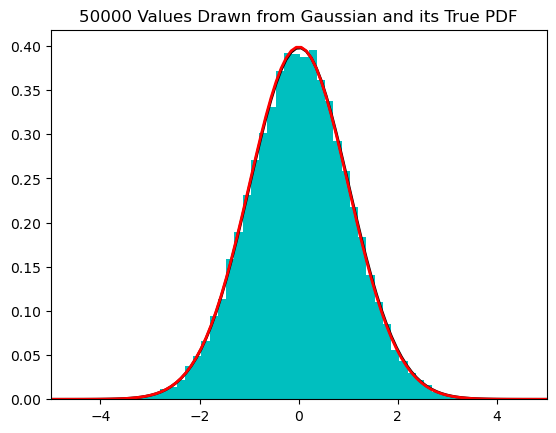
\includegraphics[scale=0.8]{gaussian.png}
  \caption{PDF of the Gaussian distribution overlaid with the distribution generated from ProbaML.}
  \label{fig:gaussian_graph}
\end{figure}

\begin{figure}[hbt]
  \centering
  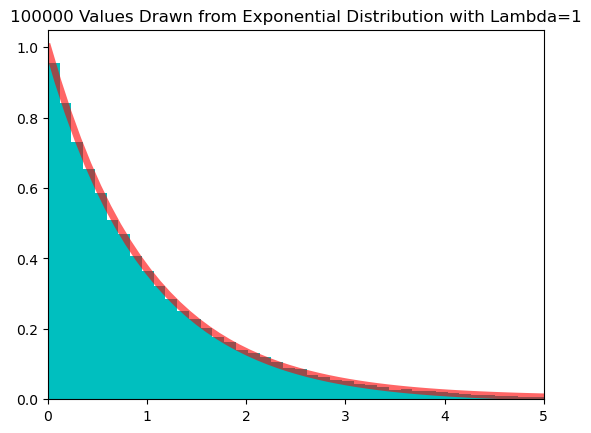
\includegraphics[scale=0.8]{exponential.png}
  \caption{PDF of the exponential distribution overlaid with the distribution generated from ProbaML.}
  \label{fig:expon_graph}
\end{figure}

\section{Future Work and Conclusions}
The project presents a clear and concise example of building a programming language from first principles and can be a useful educational tool.

Future work includes extending the project with more features, such as computing expectations with Monte Carlo simulations and support for probabilistic data structures like Bloom filters and Kalman filters. We can also extend the deterministic features of the language to support a wider array of features such as monads, custom data types and constructors, and type inference.

\newpage
\bstctlcite{bstctl:etal, bstctl:nodash, bstctl:simpurl}
\bibliographystyle{IEEEtranS}
\bibliography{references}
The GitHub repo with the code for the implementation of ProbaML can be found at \newline
\url{https://github.com/dannymf/daniML}. \newline \break
\textbf{Pledge:} This paper represents my own work in accordance with University regulations. \\
Daniel Friedman

\newpage
\section*{Acknowledgements}
Thank you to my adviser, Professor David Walker, for your constant support and willingness to meet every week. I gained so much from your insight and ideas and could not have accomplished what I did without your help.

-------------------------------------------------------------------------------------------------------------------

On a personal note, thank you Mommy for your love and encouragement always. I know I can always call you whenever I need advice or a hug (even from a distance!).

Thanks to my sister Miriam for always being there for me and for your constant calls. I know how much you care about me and that makes me feel so special. Thank you Yair for being the best brother-in-law I could've asked for. I love you so much.

Thanks to my brother Shlomo for our friendship. I really enjoy spending time together and hearing your beautiful Divrei Torah. It inspires me to see your commitment and devotion to Chesed and true friendship and connection.

Thank you Poppy for always believing in me and being a hero. I've never seen a grandfather so courageous and generous like you.

Thank you Ty for being the best roommate, and always listening and supporting me throughout my journey.

Thanks to all my friends, especially Joseph for always spending time with me, and thanks Adira for letting me share Joseph with you. Thank you both for your friendship and encouragement always.

Thanks to Nicole for helping and encouraging me through this process, and always being there to listen. I really appreciate that you always reach out and care so much.
\end{document}